\documentclass{article}
\usepackage[utf8]{inputenc}
\usepackage{graphics}
\usepackage{subcaption}


\title{Build, Test and Reporting System Report}
\author{Ashish Kumar}
\date{}

\begin{document}
\maketitle

\begin{figure}
\centering
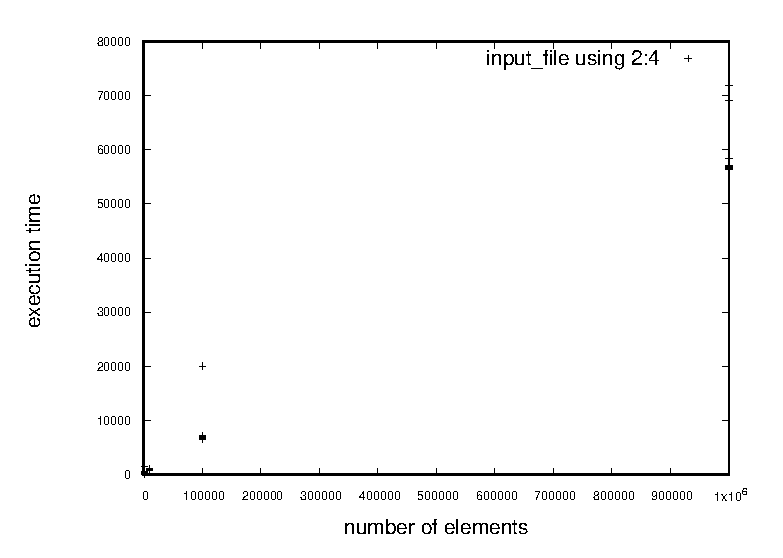
\includegraphics{graphs/1_t1.eps}
 \vspace{60pt}
 \caption{This is point scatter graph for 1 thread .}
 \vspace{30pt}
 One point (scatter) graph for thread=1 where X-axis is num-of-elements and Yaxis
 corresponds to execution time for each sample.
 \label{fig:1_t1}
\end{figure}


\begin{figure}
\centering
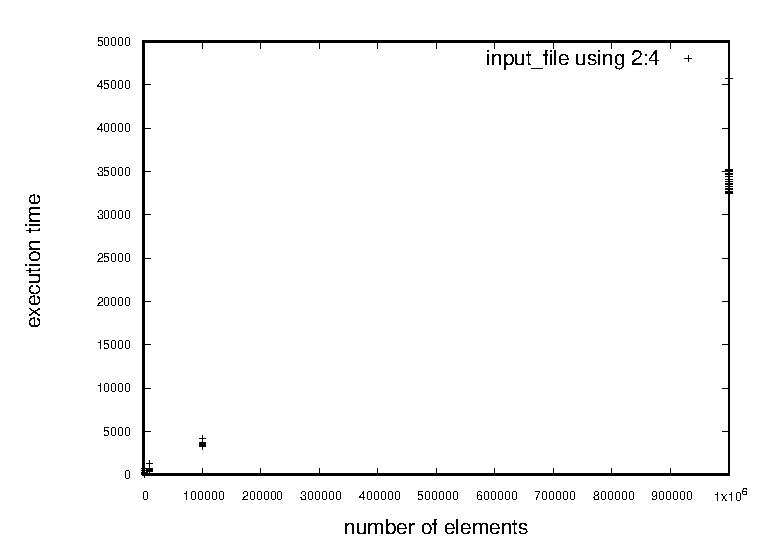
\includegraphics{graphs/2_t1.eps}
 \vspace{60pt}
 \caption{This is a scatter graph for 2 threads .}
 \vspace{30pt}
 One point (scatter) graph for thread=2 where X-axis is num-of-elements and Yaxis
 corresponds to execution time for each sample.
 \label{fig:2_t1}
\end{figure}


\begin{figure}
\centering
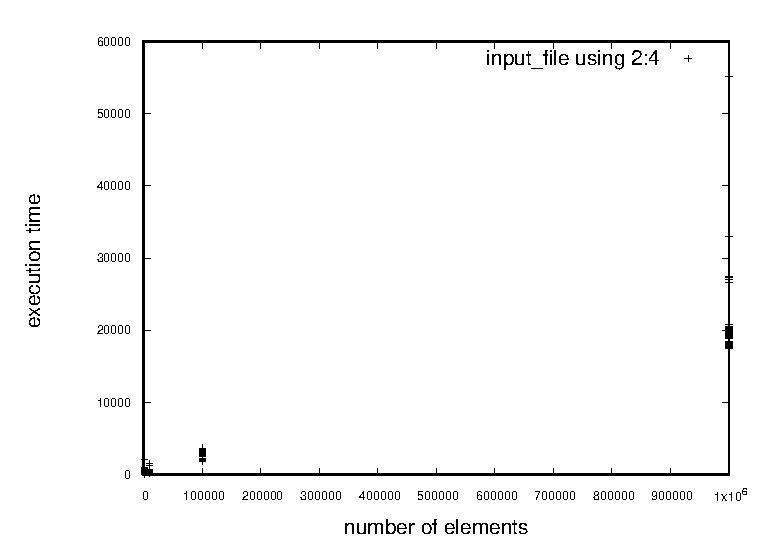
\includegraphics{graphs/4_t1.eps}
\vspace{60pt}
 \caption{This is a one point scatter graph for 4 threads .}
 \vspace{30pt}
 One point (scatter) graph for thread=4 where X-axis is num-of-elements and Yaxis
 corresponds to execution time for each sample.
 \label{fig:4_t1}
\end{figure}


\begin{figure}
\centering
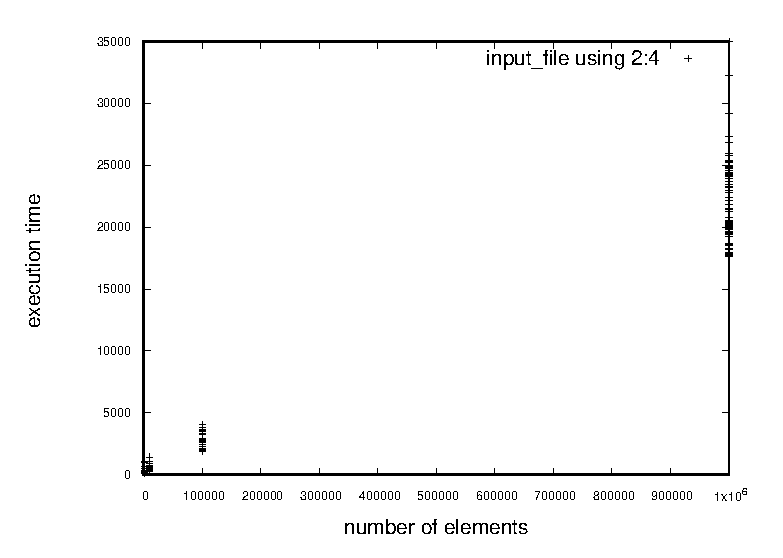
\includegraphics{graphs/8_t1.eps}
\vspace{60pt}
 \caption{This is a one point scatter graph for 8 threads .}
 \vspace{30pt}
 One point (scatter) graph for thread=8 where X-axis is num-of-elements and Yaxis
 corresponds to execution time for each sample.
 \label{fig:8_t1}
\end{figure}

\begin{figure}
\centering
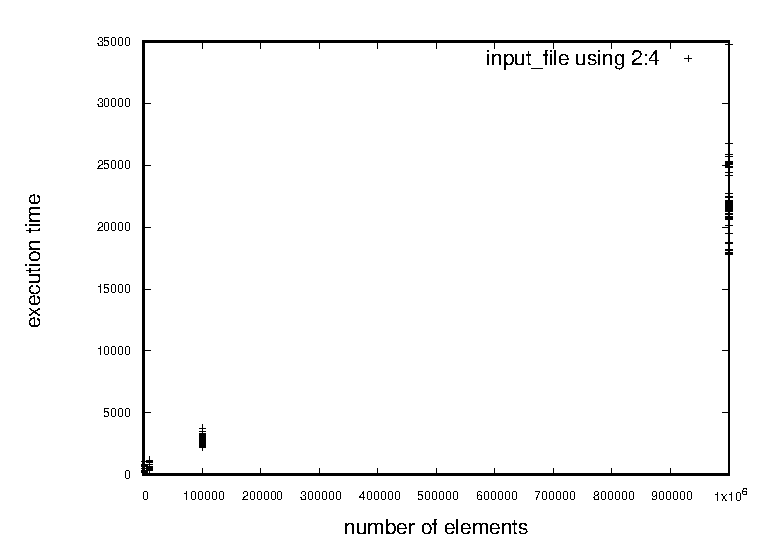
\includegraphics{graphs/16_t1.eps}
\vspace{60pt}
 \caption{This is a one point scatter graph for 16 threads .}
 \vspace{30pt}
 One point (scatter) graph for thread=16 where X-axis is num-of-elements and Yaxis
 corresponds to execution time for each sample.
 \label{fig:16_t1}
\end{figure}




\begin{figure}
\centering
\includegraphics{graphs/t2.eps}
\vspace{60pt}
 \caption{This is line graph for all threads .}
 \vspace{30pt}
 A single line graph for each thread configuration where X-axis is num-of-elements and Y-axis is
 average execution time over 100 samples
 \label{fig:t2}
\end{figure}



\begin{figure}
\centering
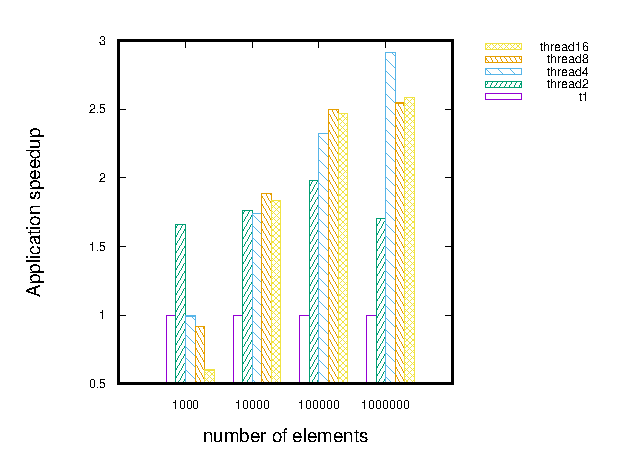
\includegraphics{graphs/t3.eps}
\vspace{60pt}
 \caption{This is bar graph for all threads .}
 \vspace{30pt}
 One bar graph with X-axis as number of elements and Y-axis as average speedup  w.r.t. one thread execution.
 \label{fig:t4}
\end{figure}

\begin{figure}
\centering
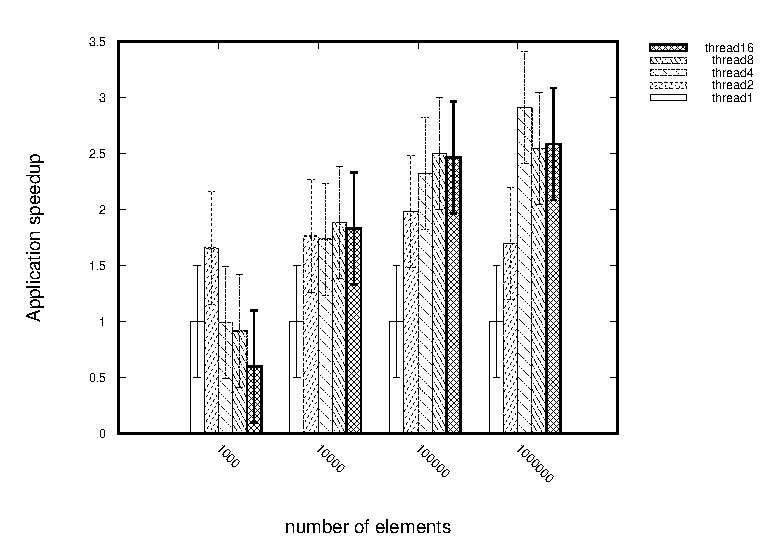
\includegraphics{graphs/t4.eps}
\vspace{60pt}
 \caption{This is bar graph for all threads with error terms .}
 \vspace{30pt}
 One bar graph with X-axis as number of elements and Y-axis as average speedup  w.r.t. one thread execution with error bars.  Where error bars represent the variance calculated
over 100 samples for a particular configuration.
 \label{fig:t4}
\end{figure}


\end{document}
